\documentclass{standalone}
\usepackage{tikz-network}
\begin{document}
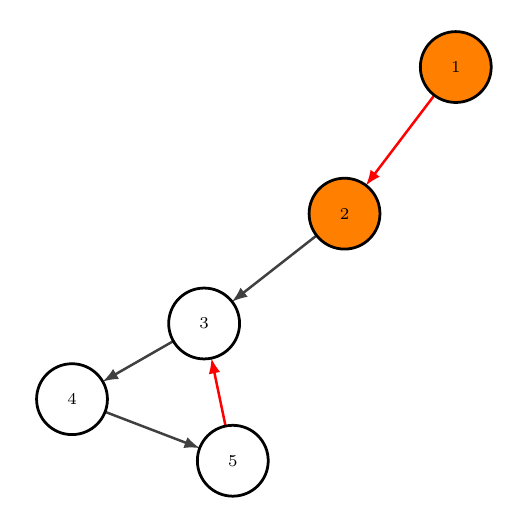
\begin{tikzpicture}
\clip (0,0) rectangle (6,6);
\Vertex[x=5.437,y=5.500,size=0.9,color=orange,label=1,fontscale=0.857,shape=circle]{1}
\Vertex[x=4.024,y=3.638,size=0.9,color=orange,label=2,fontscale=0.857,shape=circle]{2}
\Vertex[x=2.241,y=2.243,size=0.9,color=white,label=3,fontscale=0.857,shape=circle]{3}
\Vertex[x=0.563,y=1.282,size=0.9,color=white,label=4,fontscale=0.857,shape=circle]{4}
\Vertex[x=2.605,y=0.500,size=0.9,color=white,label=5,fontscale=0.857,shape=circle]{5}
\Edge[,lw=0.9,color=red,bend=0,Direct](1)(2)
\Edge[,lw=0.9,color=,bend=0,Direct](2)(3)
\Edge[,lw=0.9,color=,bend=0,Direct](3)(4)
\Edge[,lw=0.9,color=,bend=0,Direct](4)(5)
\Edge[,lw=0.9,color=red,bend=0,Direct](5)(3)
\end{tikzpicture}
\end{document}